\newpage
\section{Results and interpretation} \label{section:result}

We use the same code for the interpretation of all lines and the meaning of the different colors are presented bellow on the figure \ref{fig:legend}.

\begin{figure}[H]
    \centering
    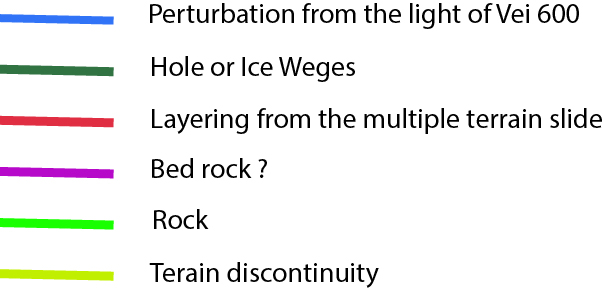
\includegraphics[width=0.5\linewidth]{Images/00_Results/Legend.jpg}
    \caption{Legend for the interpretation of the figure }
    \label{fig:legend}
\end{figure}

\subsection{Test survey}

For the test survey, survey to test the equipment, I went walking in the streets of Longyearbyen and found a very characteristics echo from pipes under the road.

\begin{figure}
    \centering
    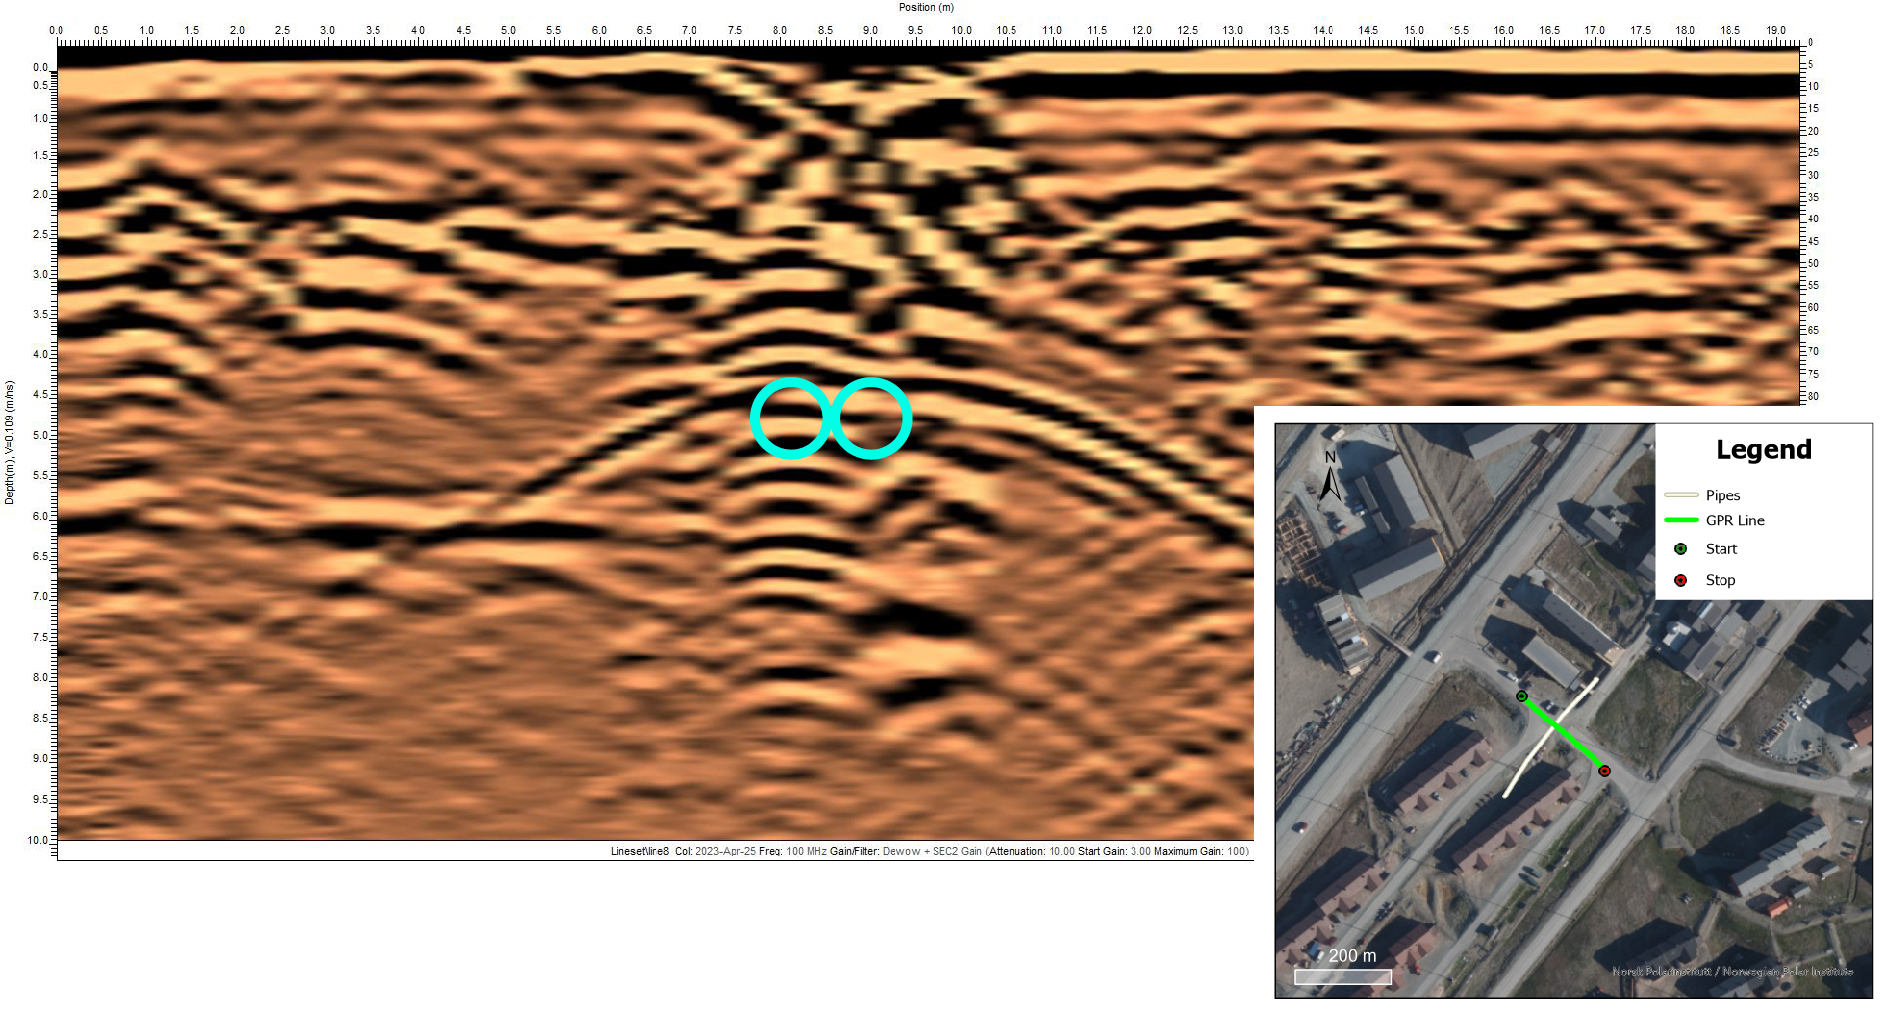
\includegraphics[width=\linewidth]{Images/00_Results/Test_line_edited.jpg}
    \caption{Test Line}
    \label{fig:testLine}
\end{figure}

The figure \ref{fig:testLine}, show a lot of small hyperbola around the position of the pipe which is very characteristics of single object buried. We also see some change in the upper layer due to the different material use for the road surface.


\subsection{Main Survey}

\paragraph{Results from the lines parallel to the slope} First we will present the lines realised parallel to the slope because they permit to understand some of the limitation of the GPR and of the ground.

\begin{figure}
    \centering
    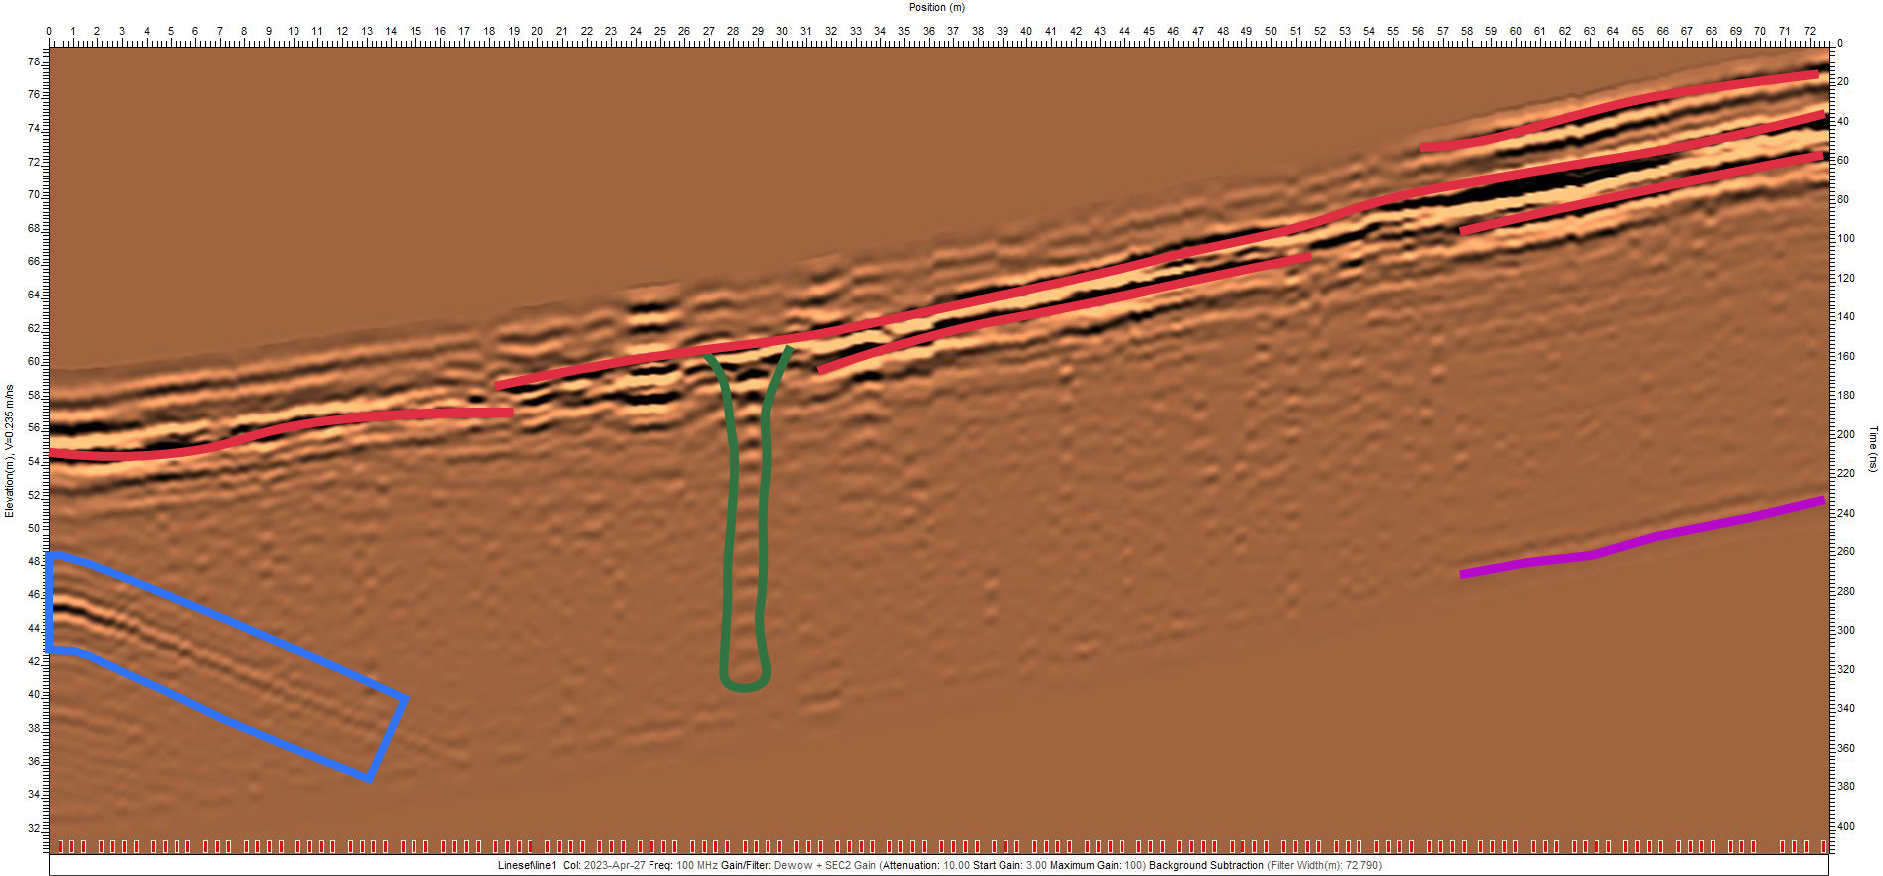
\includegraphics[width=\linewidth]{Images/00_Results/line1_edited.jpg}
    \caption{Line 1 with interpretations, legend on the figure \ref{fig:legend}}
    \label{fig:line1}
\end{figure}

\begin{figure}
    \centering
    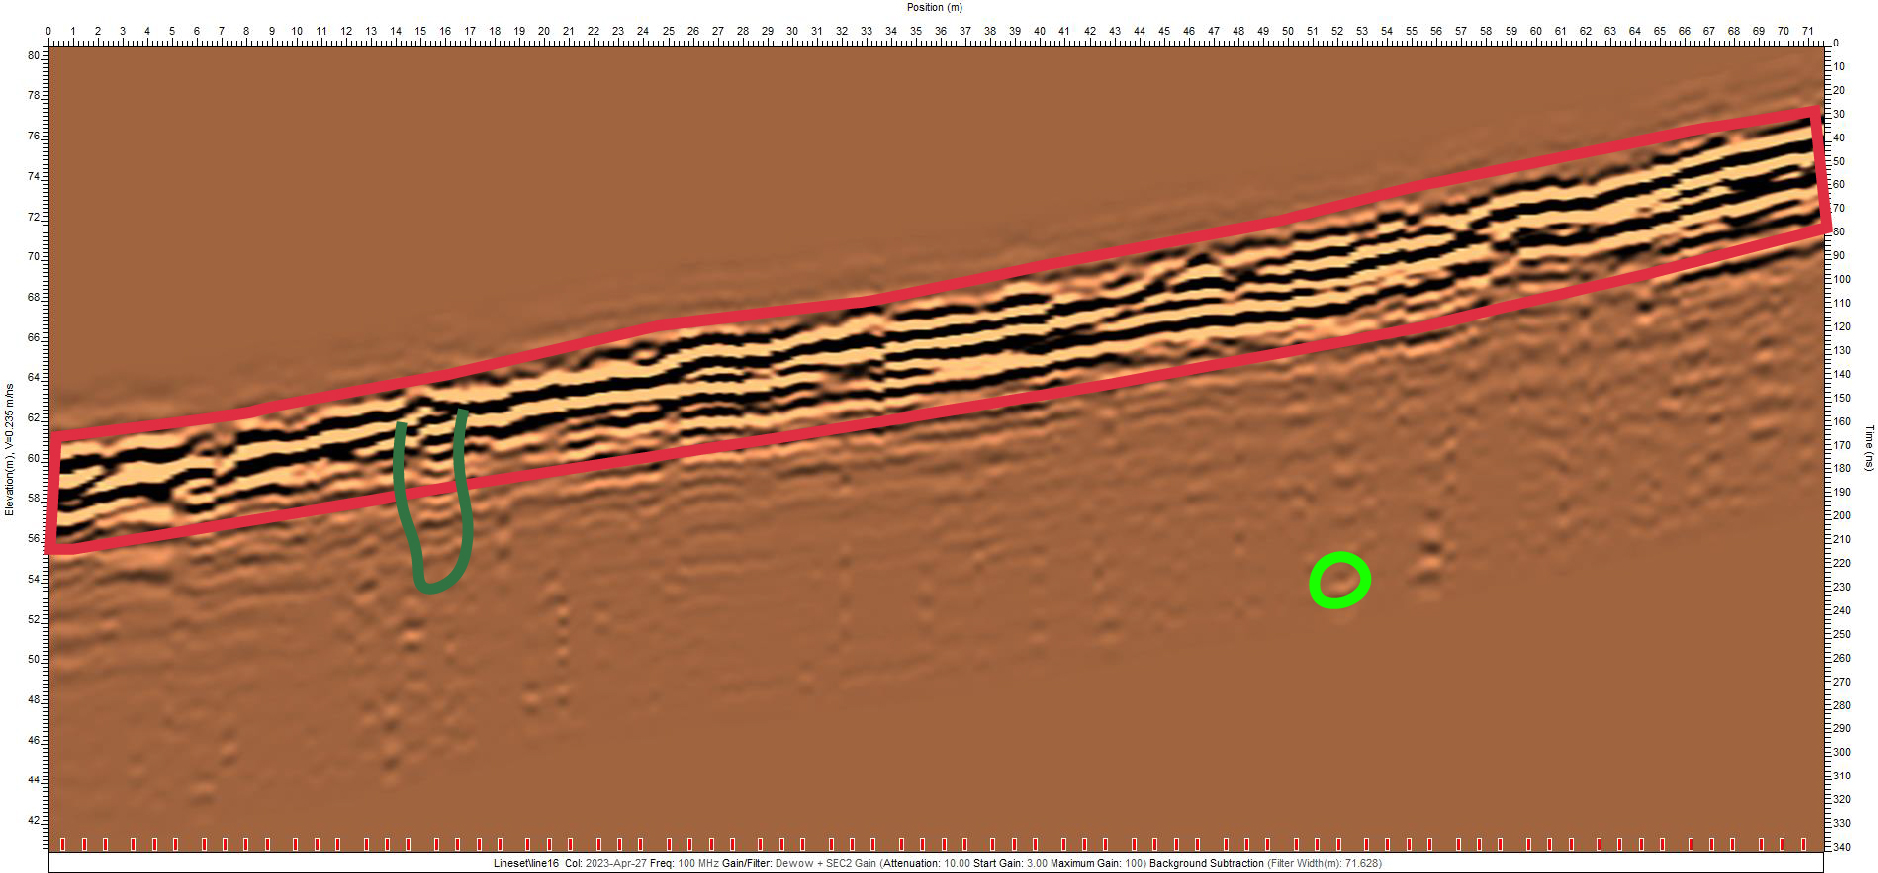
\includegraphics[width=\linewidth]{Images/00_Results/line16_edited.jpg}
    \caption{Line 16 with interpretations, legend on the figure \ref{fig:legend}}
    \label{fig:line16}
\end{figure}

\begin{figure}
    \centering
    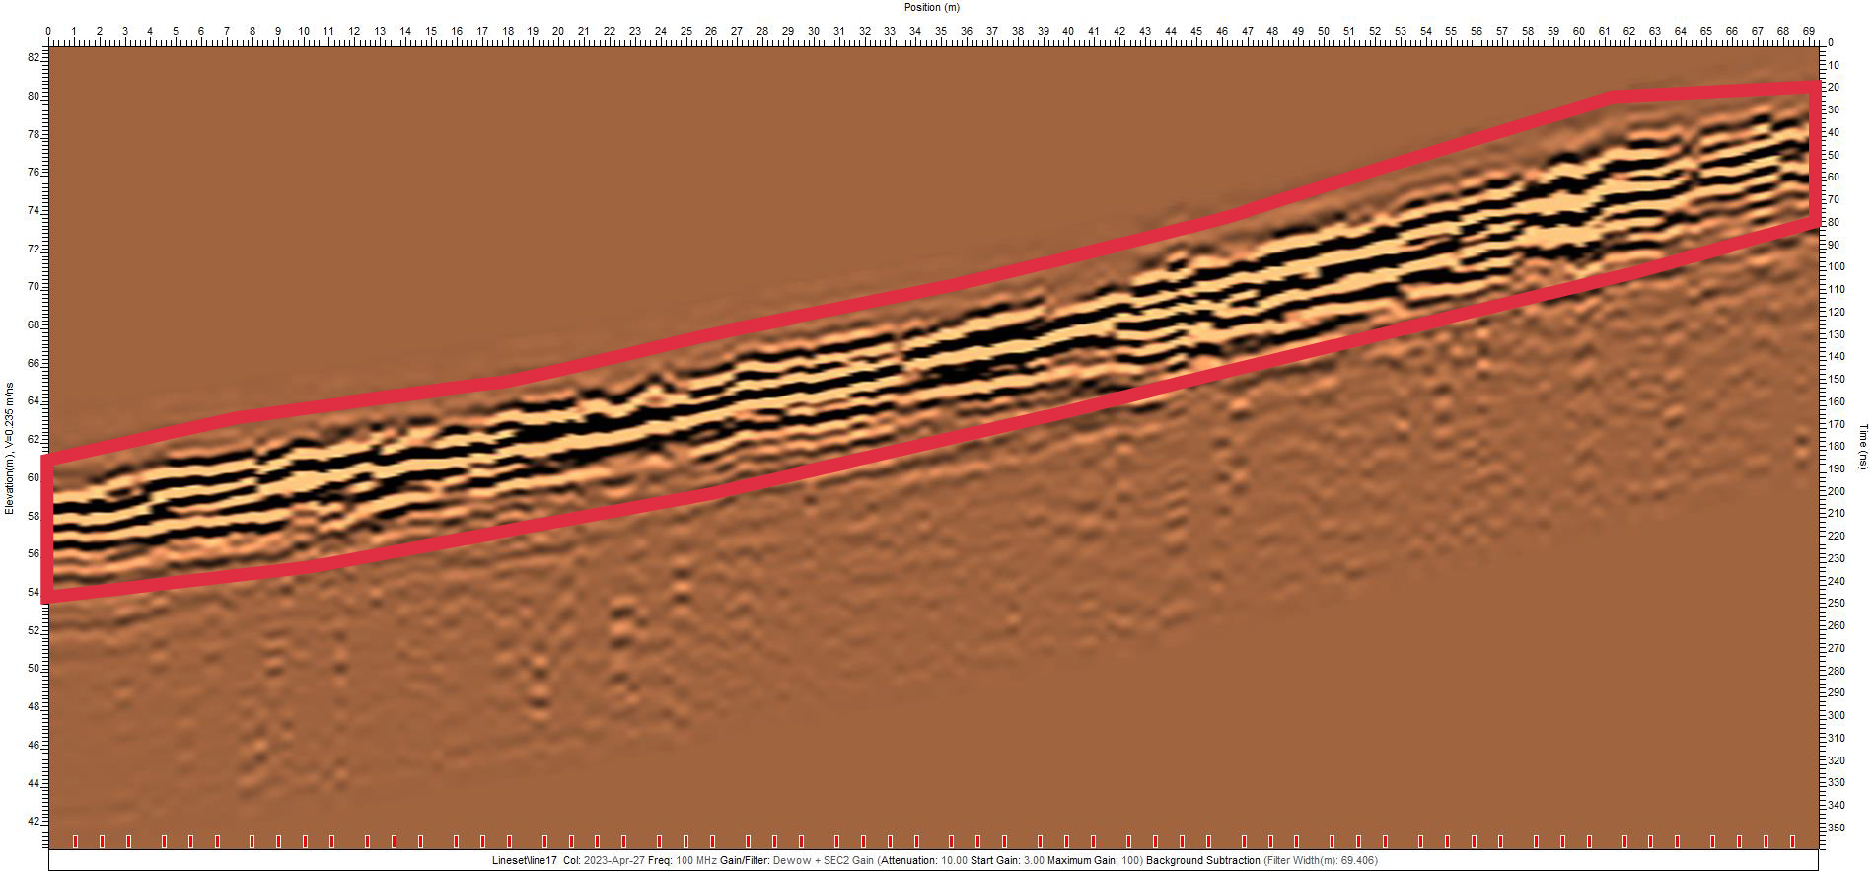
\includegraphics[width=\linewidth]{Images/00_Results/line17_edited.jpg}
    \caption{Line 17 with interpretations, legend on the figure \ref{fig:legend}}
    \label{fig:line17}
\end{figure}

\begin{figure}
    \centering
    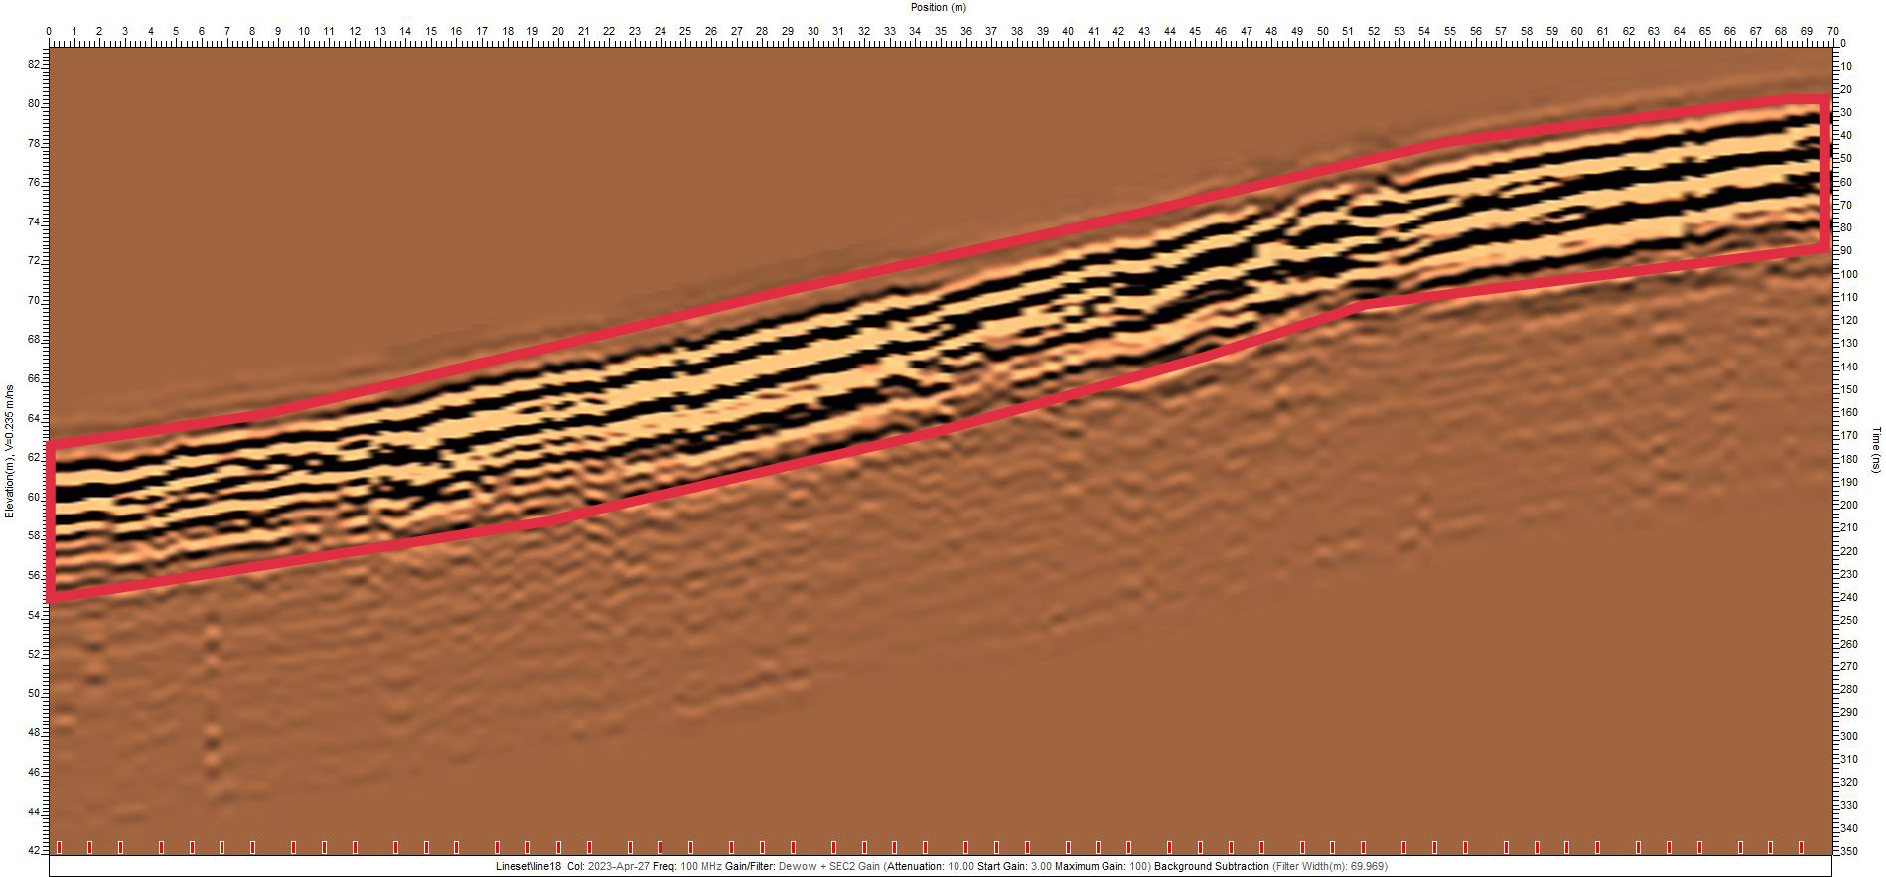
\includegraphics[width=\linewidth]{Images/00_Results/line18_edited.jpg}
    \caption{Line 18 with interpretations, legend on the figure \ref{fig:legend}}
    \label{fig:line18}
\end{figure}

\begin{figure}
    \centering
    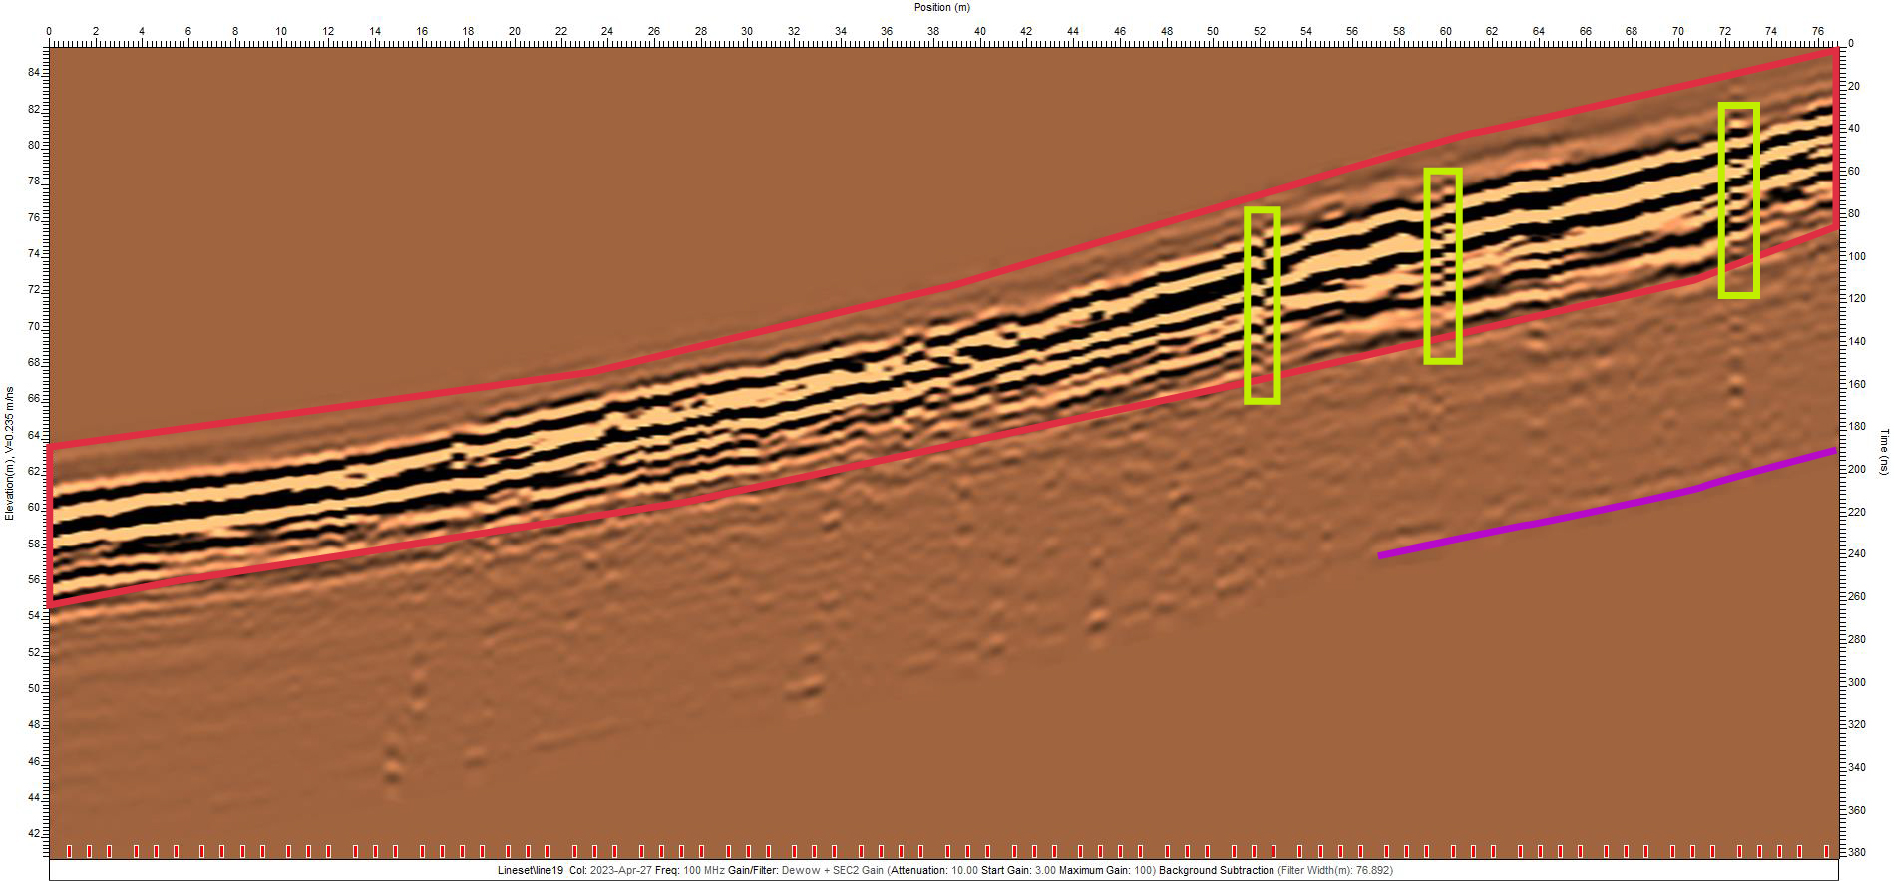
\includegraphics[width=\linewidth]{Images/00_Results/line19_edited.jpg}
    \caption{Line 19 with interpretations, legend on the figure \ref{fig:legend}}
    \label{fig:line19}
\end{figure}

\begin{figure}
    \centering
    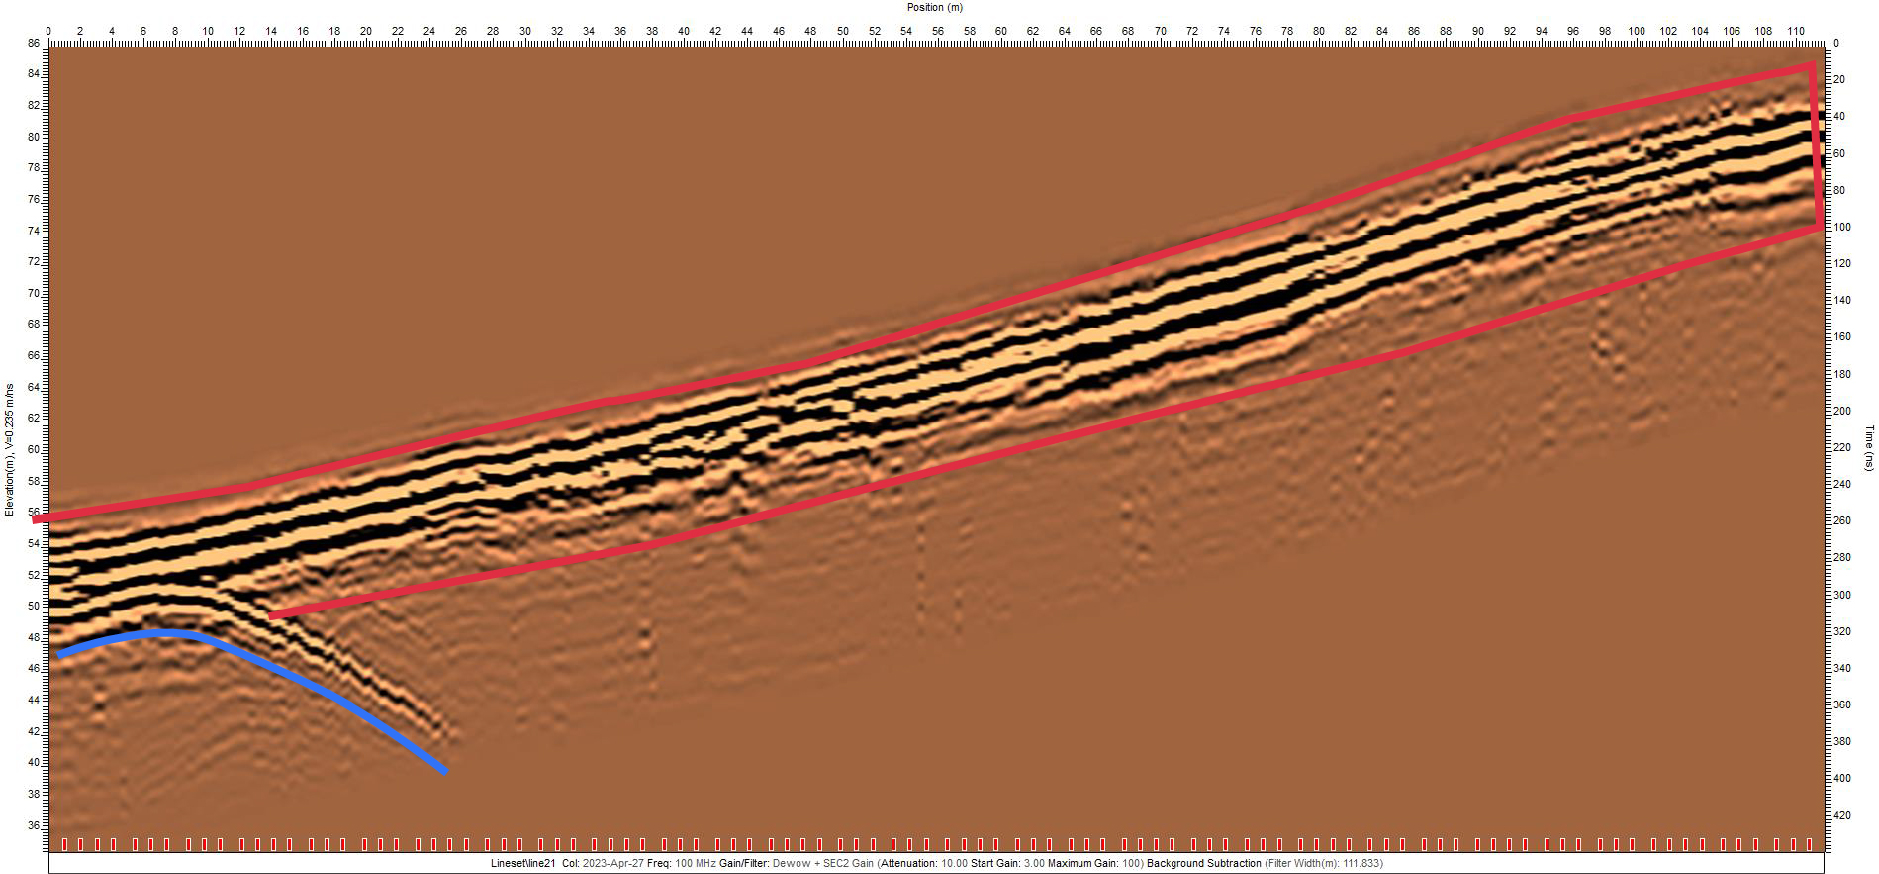
\includegraphics[width=\linewidth]{Images/00_Results/line21_edited.jpg}
    \caption{Line 21 with interpretations, legend on the figure \ref{fig:legend}}
    \label{fig:line21}
\end{figure}

